% Start of macros section

\documentclass[12pt]{article}
\setlength{\parindent}{4em}

\title{Land facets or soils: how GIS layers affect species habitat coefficients in the southern models.}
\author{Brandon Allen}
\date{September 11\textsuperscript{th}, 2019}

\usepackage[round,semicolon]{natbib}
\usepackage{color, soul}
\usepackage{graphicx}
\usepackage{amsmath}

\graphicspath{{C:/Users/beallen/Desktop/land-facet-models_2019/results/figures/}}
% End of macros section


\begin{document}

\maketitle

\section{Introduction}

The southern habitat models created by the ABMI use soil information aggregated from the AGRASID database. This database is composed of complex polygons which can contain multiple soil classes. As we don’t know how these soil classes are distributed within the polygon, we have chosen to reclassify the polygon by the dominate soil class. However, this results in lost information, and does not guarantee the soil summaries are accurate at our sites. This not only impacts the accuracy of our species models, but also our provincial and Biodiversity Data Query Tool (BDQT) predictions. An alternative to this soil layer could be the recently created land facet layer developed by Scott Nielsen. This layer categorizes 15 m\textsuperscript{2} pixels into 16 categories based on topographic features including slope, aspect, solar radiation, and wetness. With a higher spatial resolution, and a larger number of classes compared to our soil layer (16 vs 4), there may be benefits to incorporating this GIS layer into our habitat suitability modeling framework.


As this land facet layer combines several data sources, there are a few issues we should be aware of. First, the saline soils layer is derived from the AGRASID database, where polygons are defined as saline if they are greater than 30\% saline soil. This means the soil composition at our sites may be incorrect as we don’t know the distribution of saline soil in the polygon. Second, the dunes and saline soils layers have pixels masked if the topographic layers indicate the pixel is wetter or drier than expected. As we don’t have ground truthing, it makes it difficult to know which classification is correct. As Scott created the layer in a modular framework, we could choose to ignore the saline soils and/or dunes layers, or create a different rule set for stacking layers that would better meet our needs. For this initial exploration, I removed the saline soils and dunes layers and used the classification call provided by the topographic indices.


In our initial assessment, we found that on average the land facet models had a better fit than the soils based models. However, as the models included both the land cover and spatial/climate components, it was unclear as to how much the spatial/climate component was compensating for the land cover information. To address this problem, created species distribution models for 310 species of vascular plants using either the proposed land facet layer, or our current soils layer without including spatial or climate data. AUC scores for each SDM were calculated using the a complete data set, or through a leave-one-out cross validation approach. In addition, I visualized the clustering of both sets of land cover coefficients to identify how native and anthropogenic coefficients group.

\section{Results}

On average, the two land cover layers were minimally correlated (Fig \ref{fig:Corr}). However, there were instances of categories between layers which were moderately to highly correlated (e.g., TB and warm slopes, LenW and water, etc). There were 259 species models which had significantly improved model fit (red) using the land facet layer, while 42 species models exhibited no change (black), and 9 species models have significantly worse fit (blue; Fig \ref{fig:AUC}). When performing the cross-validation, the number of models which significantly improved dropped to 117, while 157 remained similar, and 36 performing significantly worse (Fig \ref{fig:CV}).

Coefficients for human footprint classes clustered in a similar patterns for both land cover layers (Fig \ref{fig:facetPCA}, \ref{fig:SoilPCA}), with Crops, Hard Linear, Urban Industrial, and Soft linear features clustering. In addition, tame and Rough pasture was more similar to native coefficients in both scenarios. Native soil coefficients were highly clustered (Fig \ref{fig:SoilPCA}), whereas native land facet coefficients clustered into two groups: sloped wet/mesic and mesic, dry, warm/cool slopes (Fig \ref{fig:facetPCA}).

\section{Discussion}

Scott's land facet data performed significantly better than our current soil land cover layer for the majority of species. In addition, we observed less clustering of land facet coefficients than the soil coefficients, suggesting the layer is capturing additional variation on the landscape. Incorporating this layer into our species modeling framework would be beneficial, but there is a lot of work that is required to accomplish this. First, this layer would need to be incorporated into Eric's workflow, where we would require land facet summaries for all ABMI sites (plus BAM), and a new back-filled layer. Second, we would need to discuss the rule set for creating a back-filled layer using this information. Third, the SC would need to update all processing scripts, including habitat summaries, species distribution models, figures, and Cure4Insect. Fourth, as the land facet layer is raster data, we need to discuss how this will impact the BDQT tool which is currently polygon based. Finally, all of these updates would need to consolidated by the IC for presentation on the website (i.e., new figure templates, definitions for coefficients). This type of update should only be implemented during a future All-In-One analysis project as it is out of the scope for a quick one off patch.

\begin{figure}[!htb]
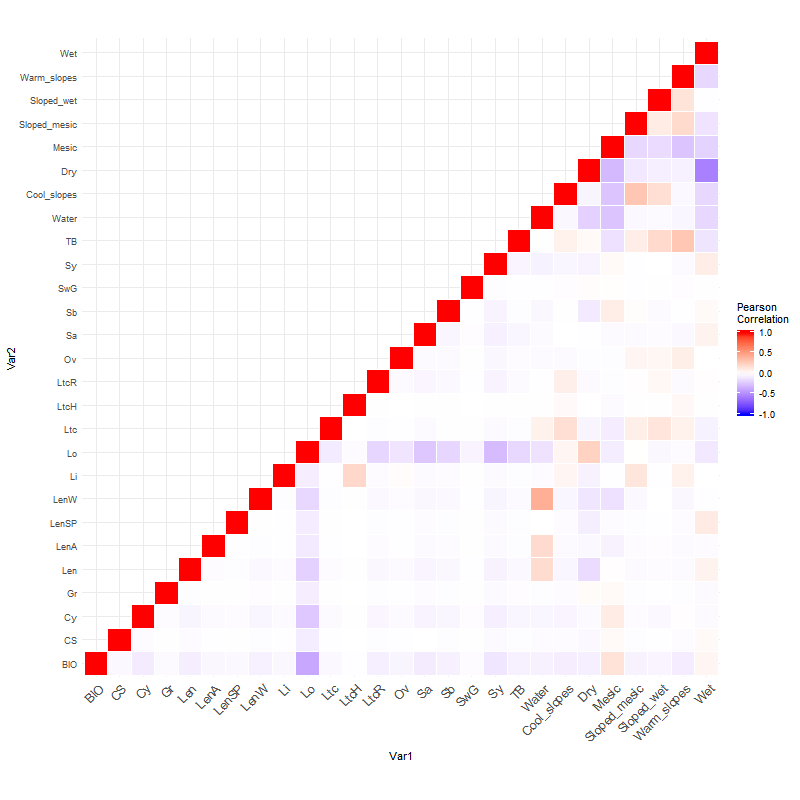
\includegraphics[scale = 0.5]{facet-soil-hf-ref_corr_2019-08-19}
\caption{Pearson correlation between the current ABMI soils layer and Scott Nielsen’s land facet layer.}
\centering
\label{fig:Corr}
\end{figure}

\begin{figure}[!htb]
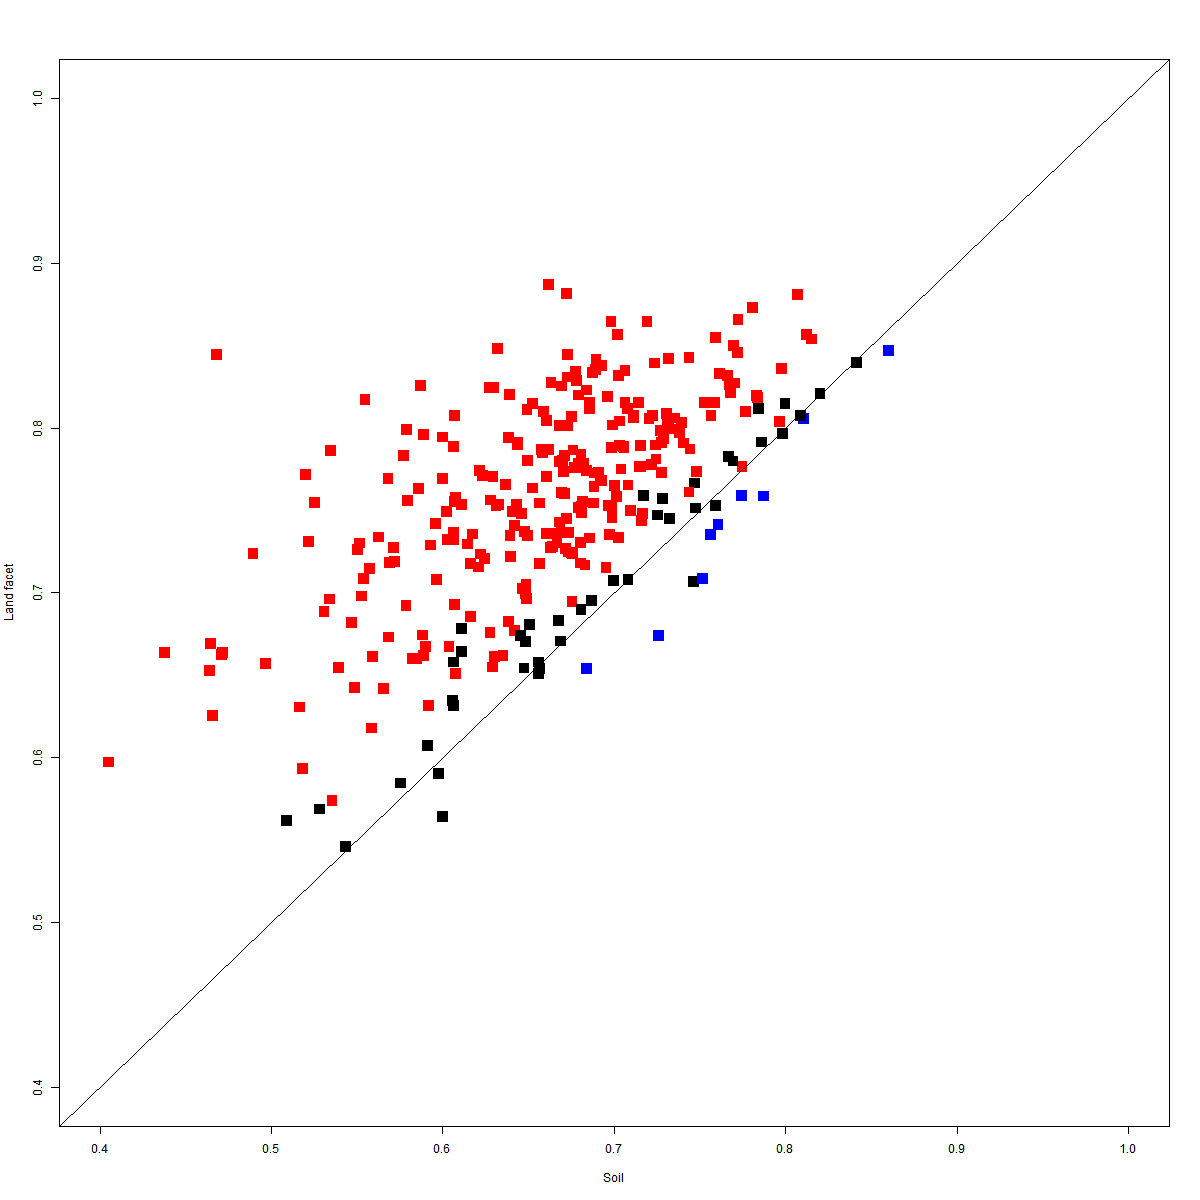
\includegraphics[scale = 0.35]{facet-soil-only-model-AUC_2019-09-04}
\caption{Comparison of AUC scores for species habitat models created using both the soils and land facet layers. Habitat models only include land cover information and do not account for the spatial/climate variation.}
\centering
\label{fig:AUC}
\end{figure}

\begin{figure}[!htb]
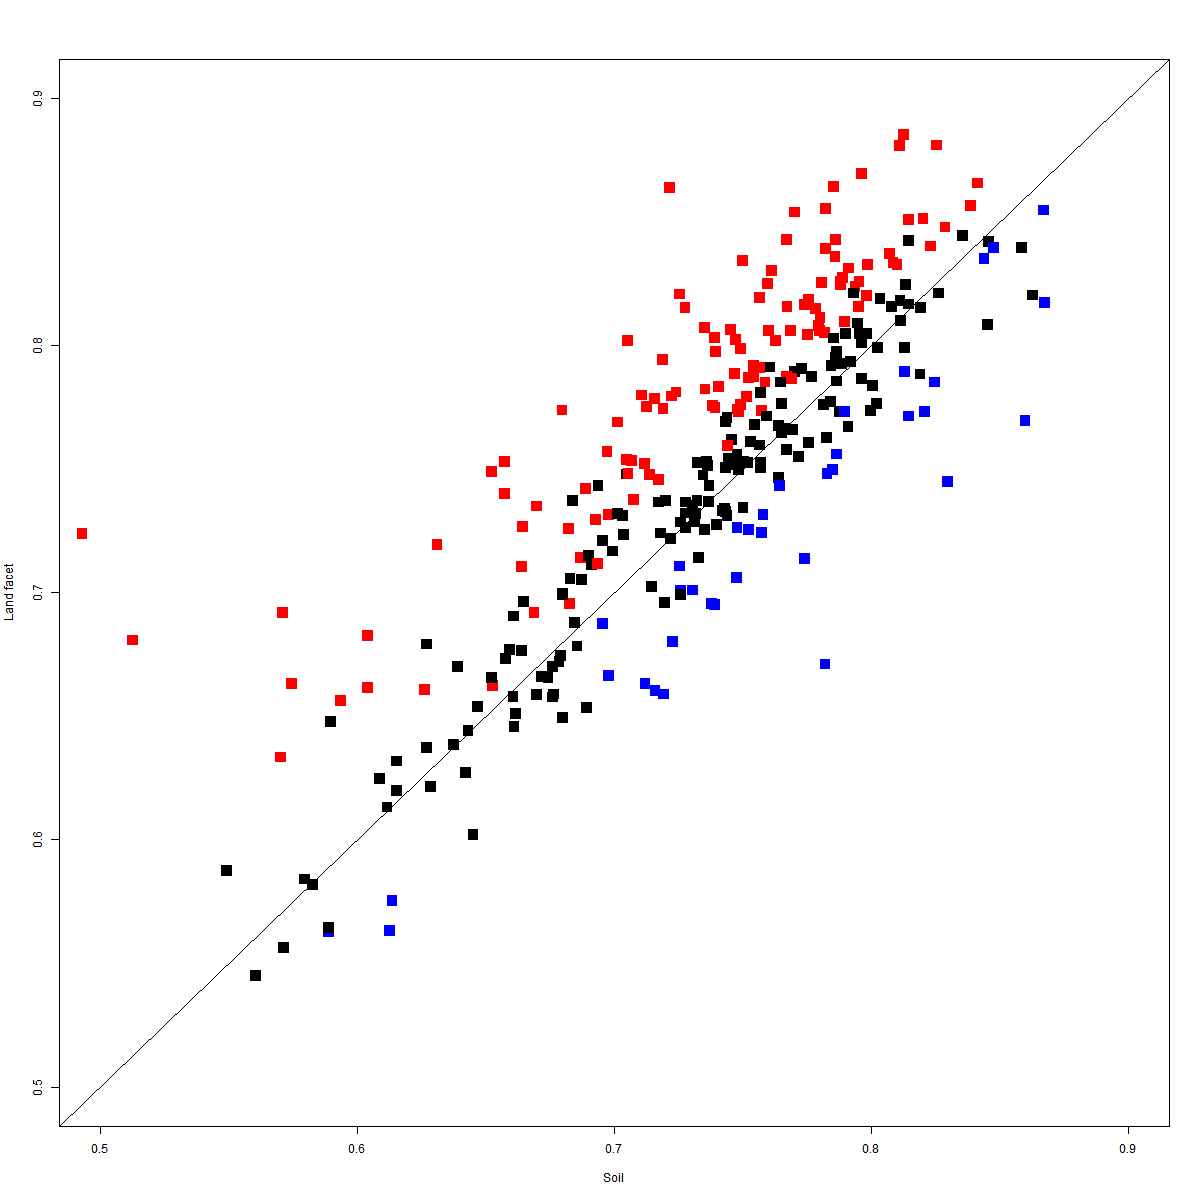
\includegraphics[scale = 0.35]{facet-soil-cv-AUC_2019-09-09}
\caption{Cross validation AUC scores of species habitat models created using both the soils and land facet layers with a leave-one-out approach.}
\centering
\label{fig:CV}
\end{figure}

\begin{figure}[!htb]
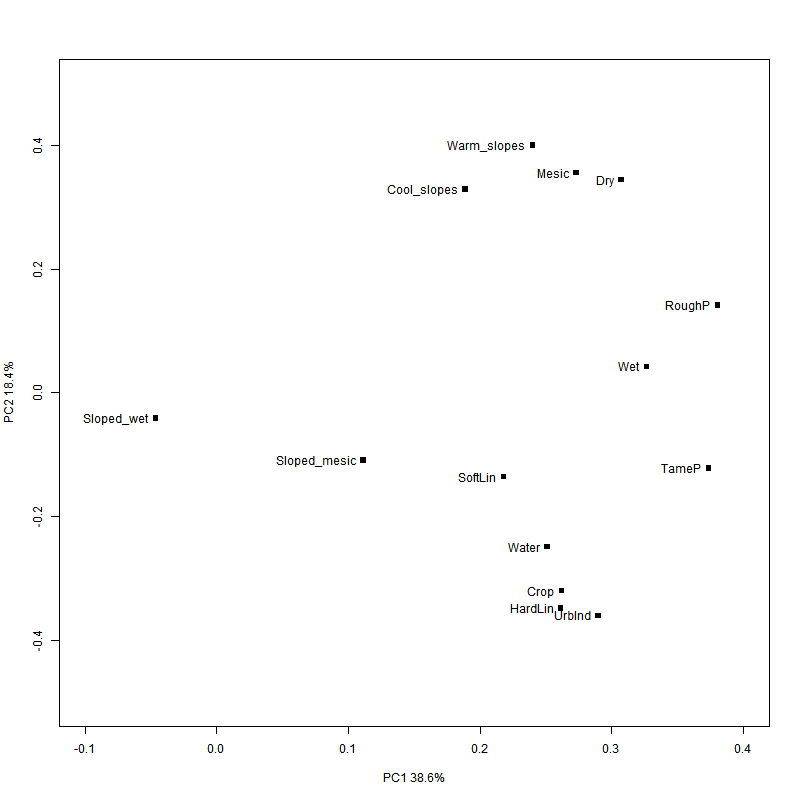
\includegraphics[scale = 0.5]{facet-pca_2019-09-04}
\caption{First two principal components of species land facet coefficients using 310 species models.}
\centering
\label{fig:facetPCA}
\end{figure}

\begin{figure}[!htb]
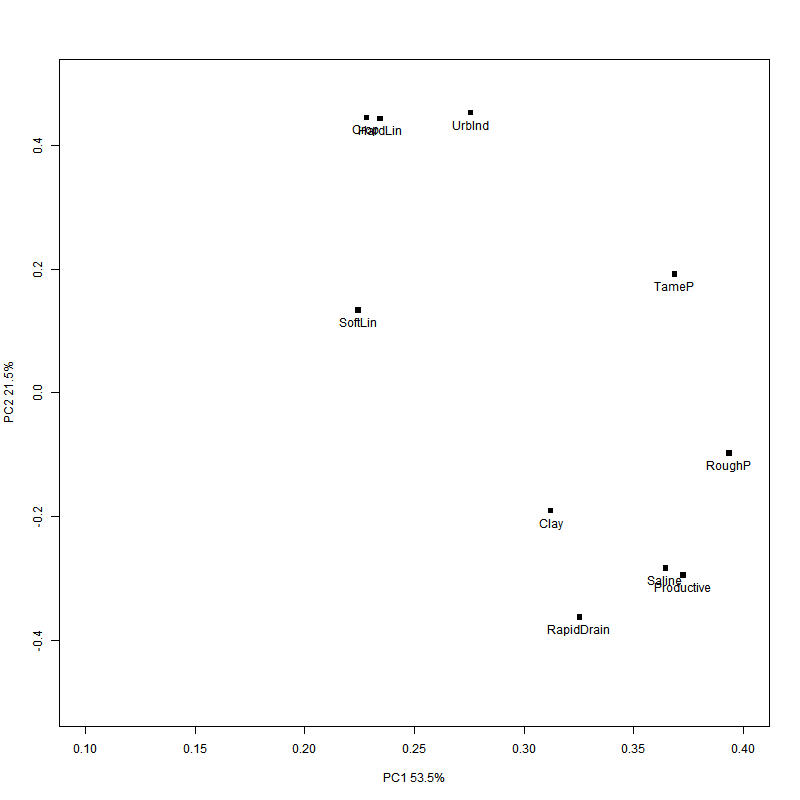
\includegraphics[scale = 0.5]{soil-pca_2019-09-04}
\caption{First two principal components of species soil coefficients using 310 species models.}
\centering
\label{fig:SoilPCA}
\end{figure}

\end{document}